%\documentclass[times, 10pt, twocolumn]{article}
%\documentclass[conference,final]{IEEEtran}

\documentclass{rspublic}

%------------------------------------------------------------------------- take
%the % away on next line to produce the final camera-ready version
%\pagestyle{empty}

\usepackage{graphicx}
\usepackage{float}
\usepackage{times}
\usepackage{multirow}
\usepackage{listings}
\usepackage{paralist}
\usepackage{wrapfig}
\usepackage[small,it]{caption}
%%\usepackage{multirow}
\usepackage{ifpdf}
\usepackage{subfigure}
\usepackage{url}

%%\usepackage{subfig}
%\usepackage[pdftex]{graphicx}
%\usepackage{harvard}
%\usepackage{pdfsync}

%Bibliography
\usepackage{natbib}
\usepackage{listings}
\usepackage{keyval}
\usepackage{color}
\definecolor{listinggray}{gray}{0.95}
\definecolor{darkgray}{gray}{0.7}
\definecolor{commentgreen}{rgb}{0, 0.4, 0}
\definecolor{darkblue}{rgb}{0, 0, 0.4}
\definecolor{middleblue}{rgb}{0, 0, 0.7}
\definecolor{darkred}{rgb}{0.4, 0, 0}
\definecolor{brown}{rgb}{0.5, 0.5, 0}
\definecolor{orange}{rgb}{1,0.5,0}

\lstdefinestyle{myListing}{ frame=single, backgroundcolor=\color{listinggray},
  %float=t,
  language=C, basicstyle=\ttfamily \footnotesize, breakautoindent=true,
breaklines=true tabsize=2, captionpos=b, aboveskip=0em,
  %numbers=left, numberstyle=\tiny
}

\lstdefinestyle{myPythonListing}{ frame=single,
backgroundcolor=\color{listinggray},
  %float=t,
  language=Python, basicstyle=\ttfamily \footnotesize,
breakautoindent=true, breaklines=true tabsize=2, captionpos=b,
  %numbers=left, numberstyle=\tiny
}

\title[Understanding Performance Implications of Distributing Data for
Data-Intensive Applications]{Understanding Performance Implications of
Distributing Data for Data-Intensive Applications}


\author[Miceli, Miceli, Rodriguez-Milla, Jha]{ Christopher Miceli$^{1}$,
Michael Miceli$^{1}$, Bety Rodriguez-Milla$^{1}$, Shantenu Jha$^{1,2,*}$ \\
\small{\emph{$^{1}$Center for Computation \& Technology, Louisiana State
University, USA}} \\  \small{\emph{$^{2}$Department of Computer Science,
Louisiana State University, USA}} \\ {\footnotesize {\hspace{0.0 in}
$^*$Corresponding Author sjha@cct.lsu.edu}} }

%\date{}

\def\acknowledgementname{Acknowledgements} \newenvironment{acknowledgement} 

% {\section*{\acknowledgementname}%\parindent=0pt% }

\newif\ifdraft \drafttrue \ifdraft \newcommand{\fixme}[1]{ { \bf{ ***FIXME: #1
}} } \newcommand{\jhanote}[1]{ {\textcolor{red} { ***Jha: #1 }}}
\newcommand{\micnote}[1]{ {\textcolor{blue} { ***Michael: #1 }}} 
\newcommand{\betynote}[1]{ {\textcolor{orange} { ***Bety: #1 }}}
\else
\newcommand{\jhanote}[1]{} \newcommand{\micnote}[1]{}\newcommand{\betynote}[1]{} \newcommand{\fixme}[1]{}
\fi

\begin{document} \maketitle

\micnote{This can't be more than 200 words. The summary should be
concise and informative. It should be complete by itself, and must not
contain references or unexplained abbreviations. It should not only
indicate the general scope of the article but also state the main
results and conclusions. Please note that footnotes are not used.}

\begin{abstract}{data-intensive computing, distributed computing,
    cloud computing, grid computing} 

  Grids, clouds and cloud-like infrastructures are capable of
  supporting a broad range of data-intensive applications. There are
  interesting and unique performance issues that appear as the volume
  of data increases which require scalable data placement and
  management techniques, as well as novel approaches to the relative
  placement of data and computational workload.  This paper aims to
  understand the factors that determine the performance of a
  representative data-intensive application, and to understand the
  performance trade-offs in design decisions. This is analogous to
  benchmarking the performance of an application on a new platform. We
  analyse two techniques to manage data placement. One focuses on data
  placement and the other on worker placement. The goal of this paper
  is to understand techniques for distributing data in a distributed
  environment and understand performance issues associated with these
  techniques.
\end{abstract}

% Grids, clouds and cloud-like
%   infrastructures are capable of supporting problems that are
%   data-intensive. There are interesting and unique performance issues
%   that appear as the volume of data increases which require scalable
%   data placement and management techniques, as well as novel
%   approaches to the relative placement of data and computational
%   workload.  The aim of this paper is to understand the factors that
%   determine the performance of a representative data-intensive
%   application, and to understand the performance trade-off in design
%   decisions. This is analagous to benchmarking the performance of an
%   application on a new platform. We analyse two techniques to manage
%   data placement. One focuses on data placement and the other on
%   worker placement. The goal of this paper is to understand techniques
%   for distributing data in a distributed environment and understand
%   performance issues associated with these techniques.

\section{Introduction} The role of data-intensive computing is
increasing in many aspect of science and
engineering~\cite{fourthparadigm}.  For example, Google, processes
around 20 petabytes of data per day ~\citep{google}, with trends
showing continuing growth. New algorithmic, infrastructure and
data-management techniques are required to handle large data-volums
effectively.  In particular at such scales data-placement and
data-scheduling need increased attention, and thus distributed
applications need to be take precautions when placing, scheduling, and
managing large volumes of data.

% As a simple example, local data-intensive applications are nearly
% always I/O bound typically dominated by Bandwidth for Cluster/Parallel
% systems, I/O dominated by latency.

The challenges in developing effective and efficent distributed
data-intensive applications are a complex interplay of distributed
applications and data-intensive applications, with different design \&
performance metrics.  For distributed systems and applications the
challenge is to find an optimal distribution strategy that takes into
account the ratio of computation workload to data distribution. Data
privacy, security and access policy are crucial issues but typically
are not determinants of performance for distributed applications.
Howeever, inefficient data placement can adversely affect system
performance greatly.  It is decisive then to determine whether to move
input data to the computational resource, or the computational
workload to the input data.

Distributed filesystems (DFS) have come of age, with multiple
open-source, reliant file-systems now available. DFS are useful and
effective tools to consider for data-intensive scientific
applications. A DFS controls the data placement and provides a uniform
interface for accessing files on multiple hosts. Thus it is worth
considering DFS as a viable infrastructure. But as the underlying
algorithms, scheduling strategies and implementations vary greatly
between different infrastructure, it is difficult to estimate {\it a
  priori} the application-level performance on a given DFS. In
general, there are many degrees-of-freedom that determine the
peformance of a given application on distributed infrastructure. Thus
a rigorous benchmarking process, which provides repeatable, extensible
and verifiable performance tests on different distributed platforms is
required.  This is analagous to the situation of developing and
testing benchmarks for high performance computing (HPC).

In this paper, we provide some initial approaches to answer ``To
distribute or not to distribute data, is the question''. Our research
focuses on understanding the performance trade-offs of a DFS compared
to ''regular'' distribution and placement techniques, as well as more
advanced intelligent distribution methods and finding how they handle
different data-sets and what the performance patterns are. This paper
also aims to determine how sensitive the performance is in the context
of a real data-intensive distributed applications.

\jhanote{Move to later section; not in introduction} In this paper, we
investigate two ways to handle this issue... \jhanote{which issue?} --
with distributed filesystems, which focus on data placement, or with
the use of an intelligent framework, which focuses on worker
placement.  .... Frequently, there is more than one copy of the input data
for fault-tolerance reasons, consequently, the added issue of deciding
between the two or more replicas becomes relevant.  While a DFS
removes the responsibility of replica management and data server
placement, the abstraction often increases the difficulty in
determining where in the DFS the data is being stored. This puts
pressure on a DFS's protocols and internal algorithms to perform
well. Despite this, the DFS replication may alleviate this issue by
placing replicas in locations where computational resources reside. A
downfall of DFSs is the inability to make the decision of whether to
move the input data, or the computational workload. It can only focus
on minimizing poor data management. The most common parameters in
determining the performance of using a DFS are the performance
overhead compared to a normal local filesystem, number of replicas of
each datum/file, and the number of servers. In our experiments, we use
the stable open source distributed filesystem CloudStore (formerly
KFS), which is written in C++ released under the Apache License
Version 2.0. It is inspired by the highly successful Google
Filesystem, GFS ~\citep{cloudstore_web}, which is closed source and
unavailable for research. CloudStore was chosen for its high
performance focus, C++ implementation, and its source code
availability. It also provides a means to automatically replicate data
on different hosts to provide efficient data access and fault
tolerance.

Our intelligent framework method differs from a DFS in that it
determines where data is and where the work should go.  Determining
data location can be as simple as looking at the IP address of the
worker and seeing geographically where it is located, or as
complicated as using network analyses tools to determine the optimal
data transfer minimization time.  For this method, we use
gridFTP\jhanote{place proper citation for gridftp}, a tool that is
used to transfer files across machines in a grid. It is specifically
designed for high-bandwidth networks.

% \section{Introduction} Data-intensive computing is a fast growing area
% of computer science. A good example of this is Google, which processes
% around 20 petabytes of data per day ~\citep{google}, and trends show
% continuing growth. It has become very important that a distributed
% application developer takes precautions when placing, scheduling, and
% managing large volumes of data. Careless placement can adversely affect
% system performance greatly. It is decisive then to determine whether to
% move input data to the computational resource, or the computational
% workload to the input data. There are two ways to handle this issue,
% with distributed filesystems, which focus on data placement, or with the
% use of an intelligent framework, which focuses on worker placement. 

% \jhanote{refine} Different metrics of concern for parallel
% vs. distributed data (I/O).  I/O typically dominated by Bandwidth for
% Cluster/Parallel systems, I/O dominated by latency. The challenge in
% load balancing for the former is often disc or bus-limited at the
% hardware level, while at the software/application level the challenge
% is to increase concurrent I/O with computation. For distributed
% systems and applications the challenge is to find an optimal
% distribution strategy that takes into account the ratio of
% computation workload to data distribution.  Data privacy, security and
% access policy is a crucial non-technical issue for distributed
% applications.  


% Distributed filesystems (DFS), motivated in part by developments in
% cloud computing, are useful and effective tools to consider for
% data-intensive scientific applications. A DFS controls the data
% placement and provides a uniform interface for accessing files on
% multiple hosts. Frequently, there is more than one copy of the input
% data for fault-tolerance reasons, consequently, the added issue of
% deciding between the two or more replicas becomes relevant. While a DFS
% removes the responsibility of replica management and data server
% placement, the abstraction often increases the difficulty in determining
% where in the DFS the data is being stored. This puts pressure on a
% DFS's protocols and internal algorithms to perform well. Despite this,
% the DFS replication may alleviate this issue by placing replicas in
% locations where computational resources reside. A downfall of DFSs is
% the inability to make the decision of whether to move the input data, or
% the computational workload. It can only focus on minimizing poor data
% management. The most common parameters in determining the performance of
% using a DFS are the performance overhead compared to a normal local
% filesystem, number of replicas of each datum/file, and the number of
% servers. In our experiments, we use the stable open source distributed
% filesystem CloudStore (formerly KFS), which is written in C++ released
% under the Apache License Version 2.0. It is inspired by the highly
% successful Google Filesystem, GFS ~\citep{cloudstore_web}, which is
% closed source and unavailable for research. CloudStore was chosen for
% its high performance focus, C++ implementation, and its source code
% availability. It also provides a means to automatically replicate data
% on different hosts to provide efficient data access and fault tolerance. 

% Our intelligent framework method differs from a DFS in that it
% determines where data is and where the work should go. 
% Determining data location can be as simple as
% looking at the IP address of the worker and seeing geographically where
% it is located, or as complicated as using network analyses tools to
% determine the optimal data transfer minimization time. 
% For this method, we use gridFTP, a tool that is used to transfer
% files across machines in a grid. It is
% specifically designed for high-bandwidth networks. GridFTP is provided by
% the Globus Toolkit, an open source software toolkit
% released under the Apache License version 2.0. Globus provides tools used
% to create and manage grid infrastructures. 

% In this paper, we provide some initial approaches to answer ``To
% distribute or not to distribute data, is the question''. Our research
% focuses on understanding the performance trade-offs of a DFS compared to
% ''regular'' distribution and placement techniques, as well as more
% advanced intelligent distribution methods and finding how they handle
% different data-sets and what the performance patterns are. This paper
% also aims to determine how sensitive the performance is in the context
% of a real data-intensive distributed applications.



\section{SAGA and SAGA-based Frameworks for Large-Scale and
  Distributed Computation}\label{Sec:SAGA}

%\alnote{removed the first paragraph - duplicated content}
% SAGA~\cite{saga_url} provides a simple, POSIX-inspired API to the most
% commonly required distributed functionality at a sufficiently
% high-level of abstraction so as to be independent of the divers\ e and
% dynamic Grid environments.

The Simple API for Grid Applications (SAGA) is an API
standardization effort within the Open Grid Forum
(OGF)~\cite{saga_gfd90}, an international standards development body
concerned primarily with standards for distributed computing. SAGA
provides a simple, POSIX-style API to the most common Grid functions
at a sufficiently high-level of abstraction so as to be independent of
the diverse and dynamic Grid environments. The SAGA specification
defines interfaces for the most common Grid-programming functions
grouped as a set of functional packages (Fig.~\ref{Fig:SAGA1}). Some
key packages are:

\begin{figure}[!ht]
 \begin{center}
     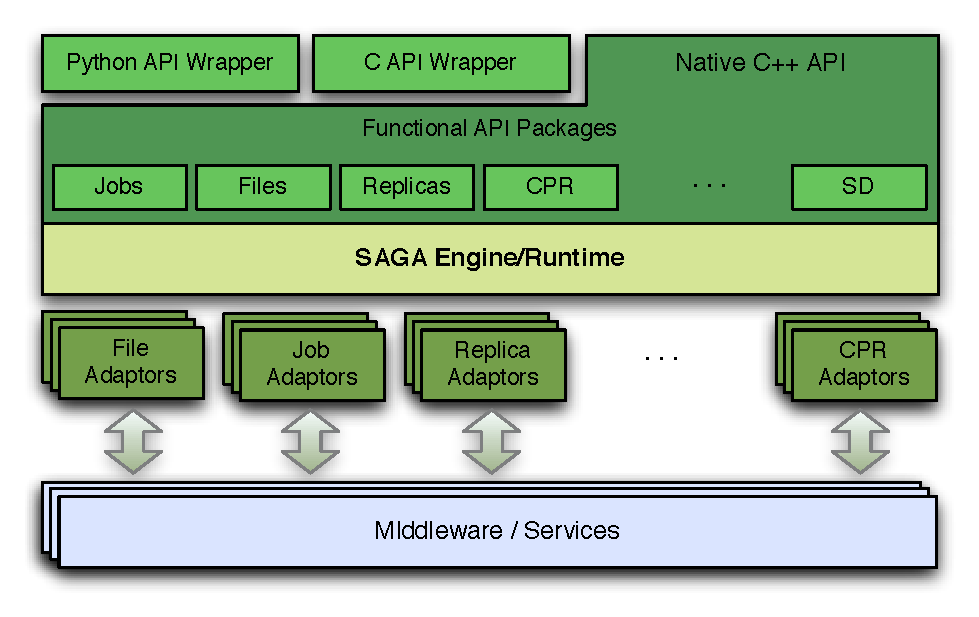
\includegraphics[width=0.40\textwidth]{stci_saga_figures-1.pdf}
    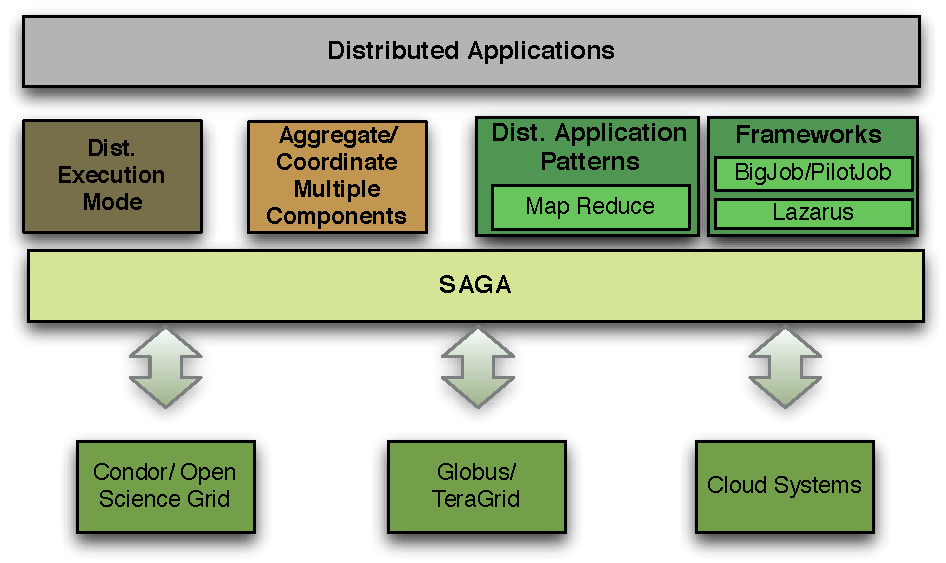
\includegraphics[width=0.45\textwidth]{distributed_applications_saga_figure.pdf}
\end{center}
\caption{\small [L] Layered schematic of the different components of
  the SAGA landscape. At the topmost level is the simple integrated
  API which provides the basic functionality for distributed
  computing. Our BigJob abstraction is built upon this SAGA layer
  using Python API bindings. [R] Showing the ways in which SAGA can be
  used to develop distributed applications.  The different shaded box
  represent the three different types; frameworks in turn can capture
  either common patterns or common application
  requirements/characteristics.} \label{Fig:SAGA1}
\end{figure}

\begin{itemize}
\item File package - provides methods for accessing local and remote
 filesystems, browsing directories, moving, copying, and deleting
 files, setting access permissions, as well as zero-copy reading and
 writing.
\item Job package - provides methods for describing, submitting,
 monitoring, and controlling local and remote jobs. Many parts of
 this package were derived from the largely adopted
 DRMAA % ~\cite{drmaa_url}                                                                                           
 specification.
\item Stream package - provides methods for authenticated local and
 remote socket connections with hooks to support authorization and
 encryption schemes.
\item Other Packages, such as the RPC (remote procedure call) and Replica
 package.
\end{itemize}

In the absence of a formal theoretical taxonomy of distributed
applications, Fig.~\ref{Fig:sagaapps} can act a guide.  Using this
classification system, there are three types of distributed
applications: (i) Applications where local functionality is swapped
for distributed functionality, or where distributed execution modes
are provided.  A simple but illustrative example is an ensemble of an
application that uses distributed resources for bulk submission. Here,
the application remains unchanged and even unaware of its distributed
execution, and the staging, coordination, and management are done by
external tools or agents. Most application in this category are
classified as implicitly distributed.  (ii) Applications that are
naturally decomposable or have multiple components are then aggregated
or coordinated by some unifying or explicit mechanism.  DAG-based
workflows are probably the most common example of applications in this
category.
% (ii) Applications that are developed using well known
% patterns, % for example MapReduce, which in turn is implemented using % infrastructure independent programming systems such as SAGA;
Finally, (iii) applications that are developed using frameworks, where
a framework is a generic name for a development tool that supports
specific application characteristics (e.g., hierarchical job
submission), and recurring patterns (e.g., MapReduce, All-Pairs).
SAGA has been used to develop system-level tools and applications of
each of these types.


% \begin{figure}[!ht]
%   \begin{center}
%     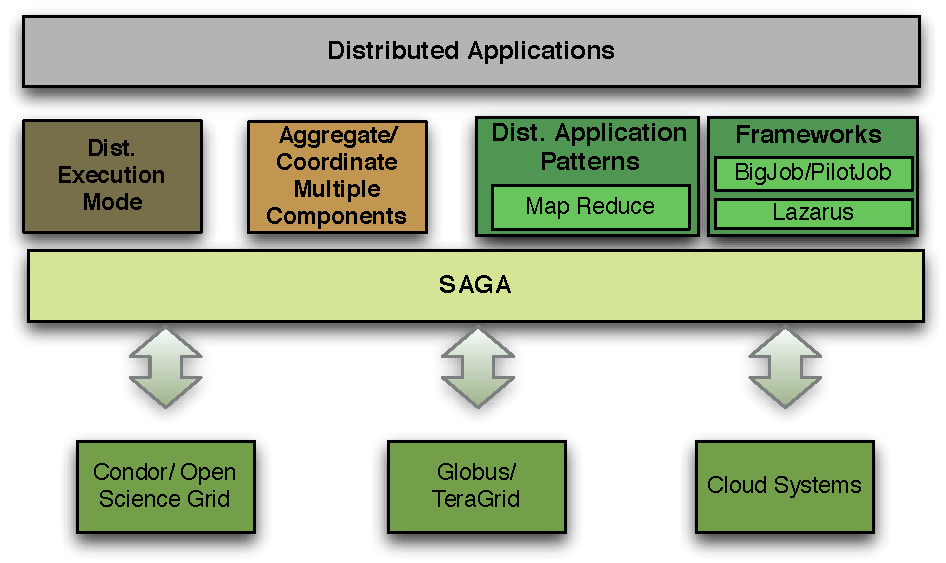
\includegraphics[width=0.45\textwidth]{distributed_applications_saga_figure.pdf}
%   \end{center}
%   \caption{\small Showing the ways in which SAGA can be used to
%     develop distributed applications.  The different shaded box
%     represent the three different types; frameworks in turn can
%     capture either common patterns or common application
%     requirements/characteristics. \label{Fig:sagaapps}}
% \end{figure}

It is important to note that SAGA provides the basic API to implement
distributed functionality required by applications (typically used
directly by the first category of applications), and is also used to
implement higher-level APIs, abstractions, and frameworks that, in
turn, support the development, deployment and execution of distributed
applications~\cite{saga_gmac09}. In Ref.~\cite{saga_montage_escience09} we
discussed how SAGA was used to implement a higher-level API to support
workflows. In this paper, we will discuss how SAGA can be used to
implement runtime frameworks to support the efficient execution of the
distributed applications.

\section{SAGA-based All Pairs: Design and Development} We use an
application based upon a grid-enabled All-Pairs abstraction in SAGA
(Simple API for Grid Applications, see Sec. \ref{Sec:SAGA}).  The
All-Pairs application was chosen because of its similarity to many
other data-intensive distributed applications.  This enables our
results to be abstracted to describe and predict different
applications besides ones based upon the All-Pairs
construct. \jhanote{a bit more describing the fact that this is a
  pattern and how benefits will be general}. This abstraction
applies an operation on two data-sets such that every possible pair
containing one element from the first set and one element from the
second set has some operation applied to it.~\citep{Interop,
  AllPairs}. Essentially, All-Pairs is a function of two sets, $A$ and
$B$, with number of elements $m$ and $n$, respectively, which creates
a matrix $M$. Each element $M_{i,j}$ is the result of the operation
$f$ applied to the elements $A_i$ and $B_j$.
\begin{eqnarray}
 AllPairs(A, B, f) & \rightarrow & M_{m \times n}, \\
\mbox{where} \quad M_{i,j} & = & f(A_{i},B_{j})
 \end{eqnarray}

The result of this application is stored in a matrix similar to Fig.
\ref{Fig:AllPairsExplanation} . The application spawns distributed jobs
to run sets of these function operations.  Examples of problems that
fall into this category are image comparison for facial recognition, and
genome comparison. This paper uses genome comparisons to find the best
matching gene in a genome. \jhanote{a bit more describing the application}.

\begin{figure}[!ht]
 \begin{center}
     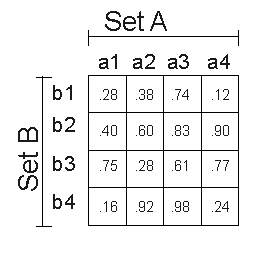
\includegraphics[width=0.50\textwidth]{data/allpairs-exp.pdf}
\end{center}
\caption{\small An example result from an All-Pairs enabled
application.  Each matrix element describes the similarity between
 the corresponding sets. (Larger values indicate more similarity.)}
 \label{Fig:AllPairsExplanation}
\end{figure}

Our genome comparison application can be classified as having a large
data throughput, as, even though it has large input $O$(GB) and
relatively small output $O$(KB), the manner of processing causes many
data reads. SAGA~\citep{saga_url} allows our application to handle
seamlessly the DFS and gridFTP based data stores on clouds and grids.
This allows the same exact application to be used for all of our
experiments. 

The problem becomes determining which pairs to put into an assignment set and
with which distributed resource to run that set. If transferring data to the
job takes too long, we spend more time on data transfer than computation.
There may be a resource capable of the work that may be slower than others,
but able to be accessed in a relatively quick manner via the network,
correcting for this lack of computational ability. An intelligent
application would attempt to predict and determine a specific data set's
affinity to a specific network resource.

%Therefore, we introduce the idea of network-closeness. A network-close
%data-set takes a small amount of time to transfer to the work location.
%A network-far data-set is just the opposite. A network-far data-set
%takes a long time to transfer to the work location. If there is an
%unprocessed data-set collocated or network-close with the job, then the
%assignment of that worker to that data-set would have benefits. If there
%is no unprocessed data-set that is network-close to the job, still we
%assign data that may be network-far, in case the network-close job
%failed or there is no available jobs network-close to the data-set.

%There are at least two types of data-intensive applications: the first
%where the actual data generated is large; the second type is where the
%data generated is small, but the volume of data on which computation
%occurs is very large. The application we used, has relatively small
%input and relatively small output, but the manner of processing causes
%many data reads. This type of application can be classified as having
%a large data throughput. \jhanote{Can you elaborate on different
%types of data-intensive applications? What kind is an ImageMagic
%based application?}


\jhanote{we need 1 paragraph about the development of adaptors for CloudStore}

\section{Performance Measurement and Analysis} We developed three types
of experiments in order to compare distributed filesystems with manual
file management. There are many questions we try to answer.  For
example, does a distributed filesystem grow more slowly than manual
placement of data?  When manually handling data, what are the advantages
of being able to move work to data to the work? For this, we find the
time to completion $t_c$, which is a function of pre-processing time
$t_x$ -- the dominant component of which is the time for transfer --,
I/O time $t_{I/O}$, which is the time it takes to read and write files,
and the time to compute $t_{compute}$, which is the time it takes for
genomes to be compared, i.e.,
 \begin{equation}
t_c = t_x + t_{I/O} + t_{compute}.
\end{equation}
We focus on three variables to measure $t_c$: degree of distribution,
data dependency, and workload. Degree of distribution is defined as
the number of resources that are utilized for a given
computation/problem. For example, if data is distributed over 3
machines $D_d$ is 3; if data is distributed over three machines but
the computational tasks over 4 machines, the $D_d$ is 4.

\subsection{Experimental Configuration}

As explained before, for our experiments, we used an All-Pairs
implementation that utilises SAGA. An XML configuration file defines
various initial parameters which alter the behavior of our All-Pairs
implementation.  Such a file defines the location of the data that
comprises the two input sets, the grouping of pairs from these sets into
sets to be provided to the compute resources, and the available machines
that will perform the operation on these sets of pairs. The application
takes these sets of pairs and maps them to a computational resource
dynamically at run-time.  

Furthermore, variables external to the All-Pairs implementation also
influence experimental results. The following experiments can be
completely described by a tuple of the following form
 \begin{equation}
(c_s, N_c, M_c, fs, m,r),
\label{Eq:tuple}
\end{equation}
where $c_s$ is the total amount of data in each file of a set (i.e.,
$c_s=\mbox{\textit{chunk} size}$); $N_c$ is the number of work-loads
that the total work is decomposed into, i.e., number of work
assignments generated; $M_c$ is a comma separated list of the machine 
configurations of the
following form: $X(c, d)$ where $X$ is a shorthand reference for the
computational resource, $c$ shows if the computational resource $X$
was used in the computational workloads/calculations, and $d$ if the
computational resource $X$ assisted in data storage, both have a
yes/no $(Y/N)$ value.; $fs$ is the type of filesystem used; $m$ is the
method used to access that filesystem; and $r$ is the degree of
replication utilized in the experiment (with a default value of 1).
 However, for CloudStore, we investigate the performance with 
 $r = 1, 2 \mbox{ and } 3$.

In our experiments, we have three $(fs, m)$ configurations, and five $X$
configurations. Our $(fs, m)$ configurations are $(L,L)=(\mbox{local,
local})$, $(L,G)=(\mbox{local, gridFTP})$, and $(C,D)=(\mbox{CloudStore,
direct})$. By direct we mean CloudStore controls the data access.
 Our $X$ configurations are enumerated in Table
\ref{Tab:Configs} below.  For one machine, $C1=X_1(Y,Y)$, where resource
$X_1$ has both the data and the computing; for two machines, we have
three configurations, and for three machines we only work with only one
configuration.

\begin{table}
\begin{center}
    \begin{tabular}{ | l | l | l |}
    \hline
    Configurations & $X(c,d)$; $c= \mbox{compute}$, $d=\mbox{data storage}$ & Description  \\ \hline
    $C1$ & $X_1(Y,Y)$  & $X_1$ computes and stores data\\ \hline    
    $C2$ & $X_1(Y,N), X_2(N,Y)$  & $X_1$ computes, $X_2$ stores data \\ \hline
    $C3$ & $X_1(Y,Y), X_2(N,Y)$  & $X_1$ computes, $X_1$, $X_2$ store data \\ \hline
    $C4$ & $X_1(Y,Y), X_2(Y,Y)$  & $X_1$, $X_2$ compute and store data \\ \hline
    $C5$ & $X_1(Y,Y), X_2(Y,Y), X_3(Y,Y)$  & $X_1$, $X_2$, $X_3$ compute and store data \\ 
    \hline
    \end{tabular}
\end{center}
    \caption{\textit{Here we show the machine configurations $M_c$ (tuple
\ref{Eq:tuple}) that we use in our experiments, for one, two, and three
machines. Both $c$ and $d$ can have yes/no (Y/N) values. A $c = Y$ means
the machine $X_i$ does computation, and a $d = Y$ means the machine has
data stored. For C4 and C5, we divide the data equally among the
machines.}}
    \label{Tab:Configs}
\end{table}

An example description of an experiment will now be explained:
 \begin{equation}
(287 \mbox{MB}, 8, C2, C, D, 1),
\end{equation}
shows that each element of a set is 287 MB in size; we have 8
assignments; the computational resource $X_1$ does calculations, but
does not have data stored, while computational resource $X_2$ does not
calculate, but stores the data; the filesystem used is CloudStore, it
directly access the files, and we have a replication factor of 1 for our
data. The machines $X_i$ we use for our experiments are in the grid LONI
(Louisiana Optical Network Initiative). For most of our experiments, the
number of assignments is 8, unless otherwise specified.  As described
above, the All-Pairs implementation used for our experiments has a fixed
distribution of data, fixed available computational resources, and fixed
sets of pairs to operate with.  These variabilities listed above (tuple
\ref{Eq:tuple}) will be manipulated to determine causes for different
I/O complexities observed in an attempt to build an understanding of
issues that arise when utilising data-intensive applications. It is also
notable that the following experiments were consistent and reproducible
for a given time, but could vary if run more than a few hours apart.
This variance is attributable to the amount of use that our computing
environment (LONI) was experiencing at the time of the experiment.

\subsection{Experiment I: Baseline Performance}
 In the first experiment, we have no actual operation begin applied on
the pairs, this is, we set $t_{compute}=0$. The reasoning behind this is to
evaluate data dependencies without the added variable of computation.
We run the SAGA-based All-Pairs application on one, two, and three
unique machines on a grid (LONI), without any specific data placement
strategy; also, no replication or fault-tolerance takes place. The
application sequentially assigns sets of pairs to the first available
computational resource. All data is accessed via the gridFTP protocol.
An important fact to notice is the essentially random mapping of data
sets to computational resources based on availability. This is to mimic
a naive data-based application. In figure
\ref{Fig:ExpIConventionalLocal}, we show our results for the local and the 
distributed case (Figs. \ref{Fig:ExpIConventionalLocal:a}, and
\ref{Fig:ExpIConventionalLocal:b}, respectively). Using our All-Pairs framework
in a distributed environment has an overhead which can be noted by looking at
the scales of both graphs. In figure
\ref{Fig:ExpIConventionalLocal:a}, our local experiments, we see that working with a smaller data set ($c_s \sim 144MB$, $N_c = 8$, 1.15 GB total) takes about half the time than working with a data set double the size ($c_s = 287MB$, $N_c = 8$, 2.3 GB total). We also see that when working with the same data set size ($2.3 GB$), but partitioned differently, i.e., S0 ($c_s = 287MB$, $N_c = 8$) vs. S1 ($c_s = 144MB$, $N_c = 16$), we increase $t_c$ for S1, by adding transfer time by doubling the number of files, although we decrease the file size by half. \betynote{Only transfer? I/O is the same, right?}In figure \ref{Fig:ExpIConventionalLocal:b}, where we use gridFTP 
to access the files, we see that a single 
machine takes less time compared to the configurations that
involve two machines. Also, having to access data remotely is a
disadvantage, $t_c(C2) > t_c(C4)$. For the number of workers $N_w$ used, we
decrease $t_c$ as we add more workers. This is, however, not true for the case
of one machine, where $t_c$ is approximately constant, probably caused by an
I/O bound.




\begin{figure}[!ht]
\begin{center}
\subfigure[ $(M_c, fs, m)=(C1, \mbox{local, local})$]{
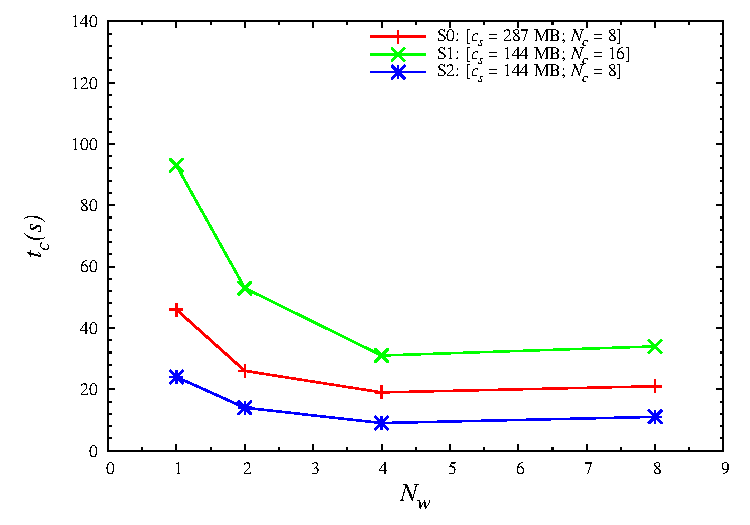
\includegraphics[scale=0.48]{data/graphs/LocalFigure}
\label{Fig:ExpIConventionalLocal:a}
}
\subfigure[$(c_s, N_c, fs, m)=(\mbox{287 MB, 8, local, gridFTP})$]{
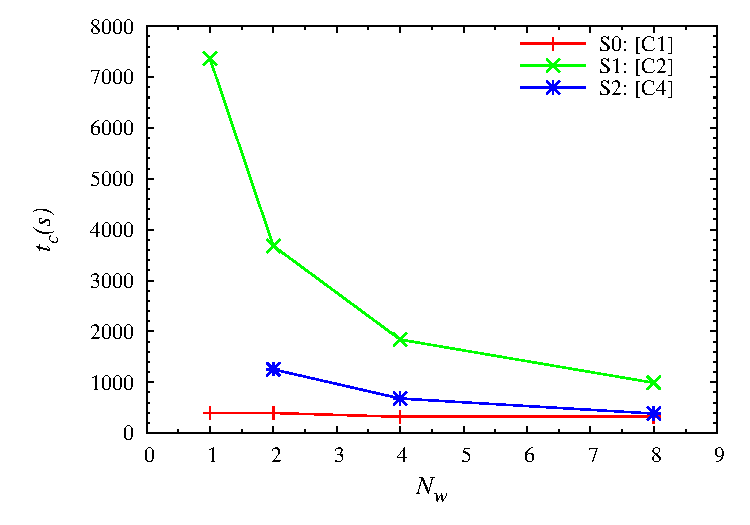
\includegraphics[scale=0.48]{data/graphs/ConventionalFigure}
\label{Fig:ExpIConventionalLocal:b}
}
\caption{\textit{Performance results for All-Pairs using gridFTP for
file reads being compared to a completely local run. We plot the time to
completion $t_c$ vs. the number of workers $N_w$. Note the scale, the
local case takes less $t_c$  than the gridFTP case. In Fig.
\ref{Fig:ExpIConventionalLocal:a}, we note that by doubling the data set size we double $t_c$, and that we create an overhead in S1 (vs. S0) by increasing $t_x$ as a result of having more files.  In Fig. \ref{Fig:ExpIConventionalLocal:b}, the two-machine
configurations take more time than using a single machine. As expected,
computing in one machine, while having the data stored in another
$(C2)$, takes longer compared to having some data stored in the resource
performing computations $(C4)$. For up to 8 workers, $t_c$ decreases as
$N_w$ increases, with the exception of a single machine where we reach
and I/O bound.}}
\label{Fig:ExpIConventionalLocal}
\end{center}
\end{figure}

%%\vspace{-0.2in}

%Bety's graph goes here
\jhanote{We need data for compute (comparison) and I/O (only) for
different data-set sizes} \micnote{We need data for three and four
machines (just one graph going from 1 machine to four machines}

%Staging experiment
\subsection{Experiment II: Intelligence Based System}
The second experiment is similar to the first, except the All-Pairs
application observes the data's location before determining whether or
not to assign a certain set of data-dependent computation to an idle
job. Inspired by earlier work~\citep{netperf}, this version of the
application performs an extra step during application startup that
approximates the performance of the network by pinging the hosts that
may be either a computational resource or a data store. This
information is then assembled into a graph data structure. This graph
is utilised at runtime when the application needs to map an idle worker
to an unprocessed set of pairs defined in the XML file. This changes the
first-available computational resource assignment mechanism described in
the first experiment to an intelligent based system. Though ping is not
very sophisticated in terms of describing a network's behavior, it is a
first-approximation to performance model aware data-placement strategy.
We also experimented with throughput via netperf \citep{netperf_web} as
a method to describe a network's behavior, but since we were working
with such a static set of resources (LONI), the same data graph was
generated as with ping. The netperf-based intelligent system took
approximately 8 seconds longer per resource to run due to the nature of
the network evaluation, but yielded no benefit. These approaches know
where the files are located and their distance to available
computational resources, thus allowing more intelligent decisions when
mapping a set of pairs to a computational resource. An even more
involved approach would be to manage locations of files dynamically at
run-time depending on usage patterns. We leave this approach to future
research.

%Figure 2

\begin{figure}[!ht]
\begin{center}
   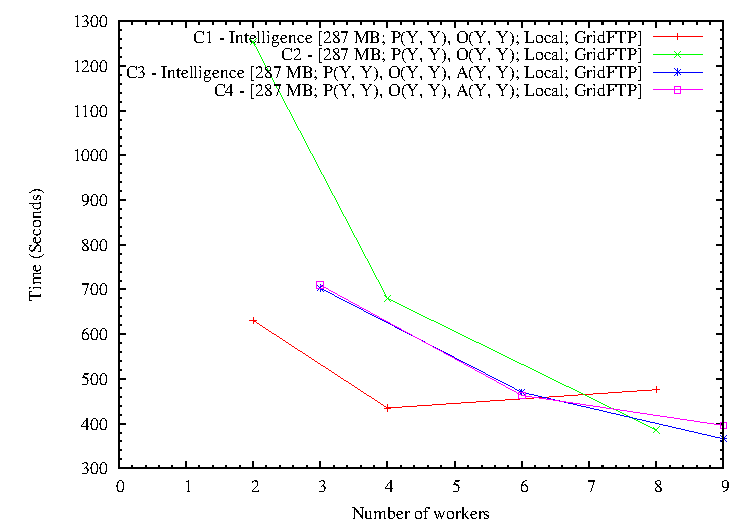
\includegraphics[scale=0.5] {data/graphs/IntelligentFigure}
\end{center}
\caption{\textit{$(c_s, N_c, fs, m)=(\mbox{287 MB, 8, local, gridFTP})$.
We compare the gridFTP and the intelligent approaches, for two and three
machines. In all cases, data is spread across all the resources.  For
the two-machine case, we observe a performance improvement by using our
intelligent approach. However, with more resources involved, out
intelligent system does not improve $t_c$.}}
\label{Fig:IntelligentExp}
\end{figure}


The overhead of intelligence includes the time spent pinging hosts and
building the graph data structure. The total time spent for this
overhead was negligible at approximately two seconds per application
run. In figure \ref{Fig:IntelligentExp}, we achieved a great reduction
in time to completion due to the use of intelligence.  However, when the
same tests were performed utilising three resources instead of two, the
intelligence seemed to offer no significant reduction. The explanation
that we propose for this, is that the sets of pairs defined in the XML
file at application start were geographically dispersed throughout the
network.  Essentially, each set of pairs had approximately the same cost
calculated by using the graph data structure. Each set of pairs would
take the same time to compute using any computational resource.
\jhanote{Perhaps define a test to verify this, so a note can go in
saying we investigated this}

\subsection{Experiment III: CloudStore} 
The third experiment provides information into CloudStore's performance
in handling data locality issues. The same All-Pairs application as in
Experiments 1 and 2 is used, except all data is stored on the
distributed filesystem CloudStore under various configurations. Some
variables of importance include number of data servers that store data,
replication value for data in these data servers, and as above,
placement and number of computational resources.  All read and writes
also utilise the distributed filesystem. Again, for our first set of
results, we focus on $t_{compute}=0$.  
%Figure 3
\begin{figure}
\begin{center}
\subfigure[One and two machines, $r = 1, 2$]
{
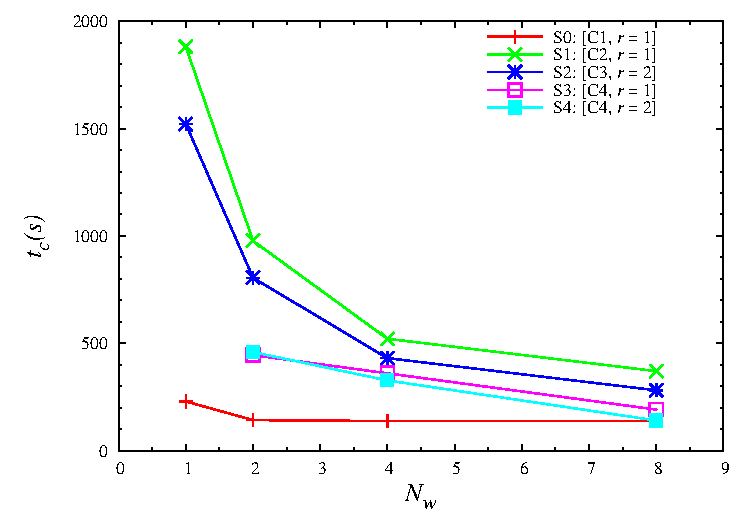
\includegraphics[scale=0.48]  {data/graphs/CloudStoreFigure}
\label{Fig:experiment3:a}
}
\subfigure[Three machines, $r = 1, 2, 3$]
{
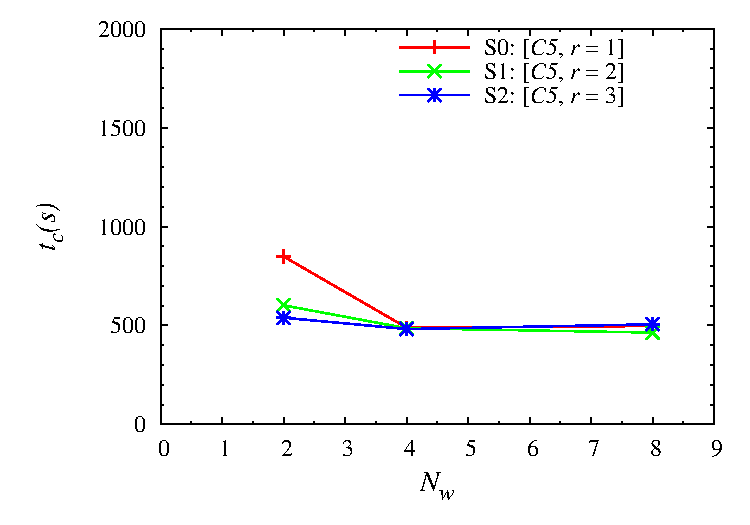
\includegraphics[scale=0.48] {data/graphs/CloudStore3Mach}
\label{Fig:experiment3:b}
}
\caption{\textit{$(c_s, N_c, fs, m) = (\mbox{287 MB, 8, CloudStore,
Direct})$. The figure on the left demonstrates All-Pairs' performance
with CloudStore locally and on two different machines. The figure on the
right demonstrates how this scales to three machines, for degree of
replication $r=1,2,\mbox{and } 3$. CloudStore performs better than our
local and intelligent approaches (see Figs.
\ref{Fig:ExpIConventionalLocal} and \ref{Fig:IntelligentExp}). Again,
having data in the resource with the workload decreases $t_c$. When data
is spread across all the computational resources, having a degree of
replication $r = 1, 2, \mbox{or } 3$ does not significantly decrease
$t_c$, except to the case of three machines and 2 workers.}
\jhanote{This caption needs attention}}
\label{Fig:experiment3}
\end{center}
\end{figure}


As done above for the first experiment, we have attempted to capture how

compute time scales under these configurations, see figure \ref{Fig:experiment3}. Having data remotely affects the performance. We can see that computing in one resource while the data is in another (S1), takes the most amount of time. Having some data in the resource that is computing helps performance (S2, S3, S4). The number of machines to which workload was assigned is also important. Placing workload in two machines also decreases $t_c$ (S2 vs. S3). We varied the degree of replication for our $C4$ and $C5$ configurations, i.e., for the case of two and three machines, where all the resources have workload assigned and data stored. In the case $C4$, having $r = 2$ improved $t_c$, but not considerably. For $C5$, different degrees of replication only made a difference in the case of two workers.

We now add our actual genome comparison function, i.e., $t_{compute} \ne 0$ and we compare it to our base case where $t_{compute} \ne 0$ . We define $\Delta t_c$ which is the time difference between these two cases. In figure \ref{Fig:experiment4}, we see that the time it takes to do the genome comparison is relatively small compared to the set up time, transfer, and I/O time added together. The fact that $\Delta t_c$ for a given $N_w$ is not the same for most of configurations, shows that there is still an overhead; our $t_x$ and $t_{I/O}$ were not the same at the times we run our All-pairs framework for both cases. \betynote{Guys, does this statement seem ``true''?}
%Figure 4

\begin{figure}
\begin{center}
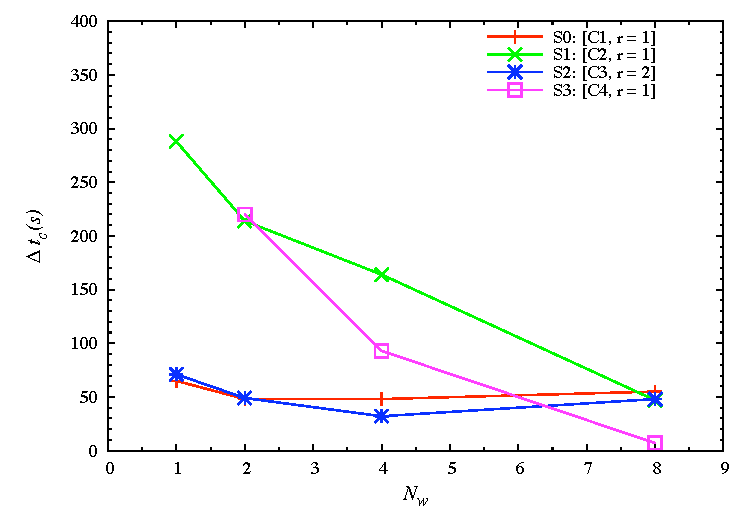
\includegraphics[scale=0.5]{data/graphs/CloudStoreComputeMinusNoCompute144}
\caption{\textit{$(c_s, N_c, fs, m) = (\mbox{144 MB, 8, CloudStore, Direct})$. Comparison of CloudStore using the All-Pairs application with and without actual computation. $\Delta t_c$ is  defined as the time $t_c(t_{compute} \ne 0)$ where we include our genome comparison function, minus $t_c(t_{compute}=0)$, where we don't include the function. For the case of $c_s=144MB$, our genome function takes about two orders of magnitude less than $t_x$ and $t_{I/O}$ combined. $\Delta t_c$ at a given $N_w$ differ for most of our configurations, showing an overhead, probably caused by different network conditions at the times our runs were performed.}}
\label{Fig:experiment4}
\end{center}
\end{figure}

We also compare our results with $t_{compute}=0$ for two different data set sizes, one with $c_s = 287MB$, and the other one with half the size, $c_s = 144MB$ (rounded value). Both use CloudStore, and have eight assignments. We define two quantities, $\Delta t_c^d = t_c(c_s = 287MB) -  t_c(c_s = 144MB)$, and $t_{O/H} = 2 \times t_c(c_s = 144MB) - t_c(c_s = 287MB)$. Figure \ref{Fig:CloudStore287minus144} shows us that there are multiple factors that can alter $t_c$. Some of the factors are network conditions, I/O time, as well as transferring time that can be size dependent, disk seek time, etc. In figure \ref{Fig:CloudStore287minus144:a}, we see that the difference does not scale linearly with the number of workers. It is worth noticing that $\Delta t_c$ is almost zero (and negative) for eight workers when all the resources have workload and data stored (C4); this is, it took about 10 seconds less for a 2.3GB set vs. a 1.15 GB set. \betynote {Why?}.  Figure \ref{Fig:CloudStore287minus144:b} shows that for most of our configurations, there is an overhead which decreases with the number of workers. It also show us that the remote data case is the one with the most overhead. Moreover, our $C4$ configuration seems to use a ``non scalable'' infrastructure, as the overhead increases with eight workers.


\begin{figure}
\begin{center}
\subfigure[$\Delta t_c^d (= t_c(287MB) -  t_c(144MB)) * N_w$]
{
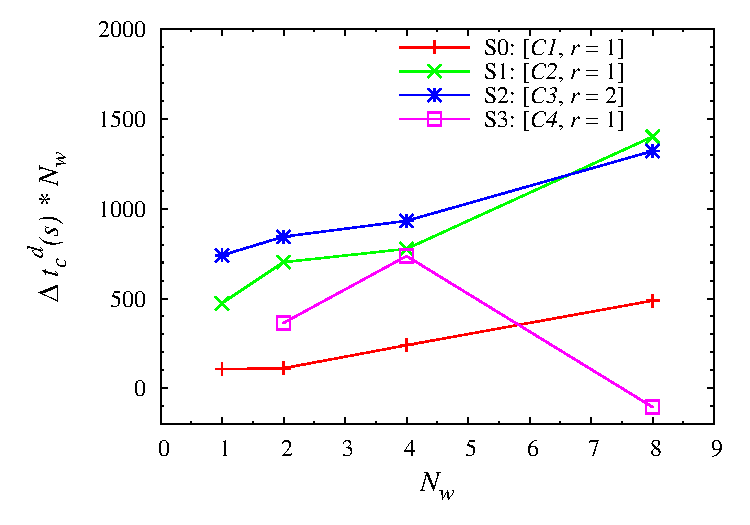
\includegraphics[scale=0.48]{data/graphs/CloudStoreNoCompute_287Minus144TimesNw}
\label{Fig:CloudStore287minus144:a}
}
\subfigure[$t_{O/H}=2*t_c(144MB)-t_c( 287MB)$]
{
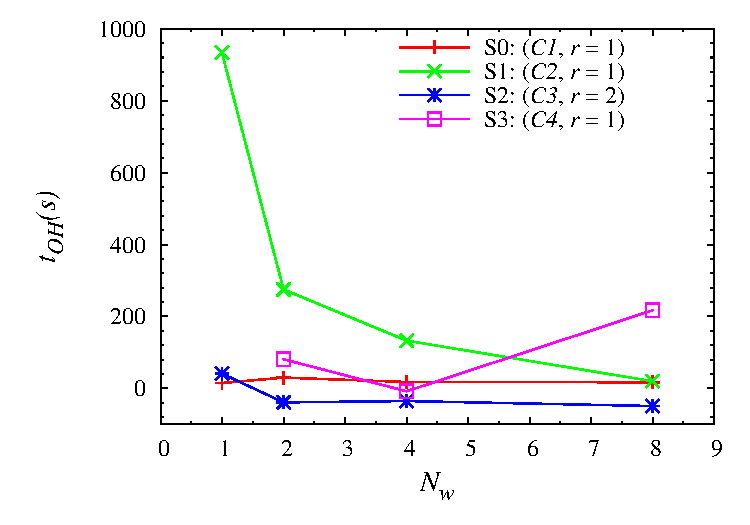
\includegraphics[scale=0.48]{data/graphs/CloudStoreNoCompute_287Minus144CommonTime}
\label{Fig:CloudStore287minus144:b}
}
%%\subfigure[$\Delta t_c$]
%%{
%%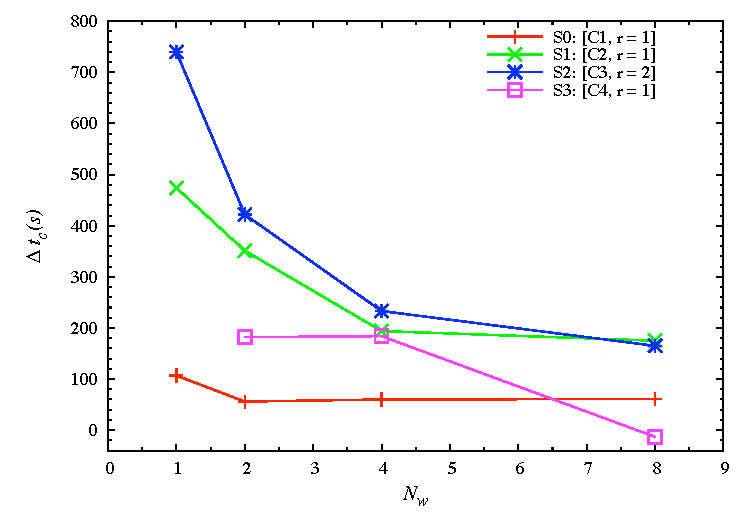
\includegraphics[scale=0.5]{data/graphs/CloudStoreNoCompute_287Minus144}
%%\label{Fig:CloudStore287minus144:c}
%%}
\caption{\textit{$(N_c, fs, m) = (\mbox{8, CloudStore, Direct})$. Here we compare $t_c$ for data set sizes 1.15 GB and 2.3 GB, this is, for chunk sizes $c_s = 144\mbox{MB and } 287\mbox{MB}$. For this, we define two quantities, $\Delta t_c^d$, which is the difference between $t_c$ found for both $c_s$'s, and $t_{O/H}$, which is the overhead time of working with chunks of 287MB in size vs. half-size chunks. In figure \ref{Fig:CloudStore287minus144:a} we see that the difference decreases with the number of workers, but does not scale linearly with $N_w$. In figure \ref{Fig:CloudStore287minus144:b}, we see that the remote data case (C2) is the one with the most overhead.}}
\label{Fig:CloudStore287minus144}
\end{center}
\end{figure}

We compared optimal times for both our intelligent approach and CloudStore as a function of the number of resources $N_r$ in figure \ref{Fig:CloudStoreVsGridFTP:a}. CloudStore performs better for one and two machines, but not for three resources, when CloudStore decreases its performance. Optimal times of our intelligent approach are about the same for $N_r=1,2,3$. In figure \ref{Fig:CloudStoreVsGridFTP:b} we plot our completion time as a function of the number of workers for three resources. All the resources have workload assigned and have data stored. CloudStore's performance did not vary significantly with the number of workers, while our intelligent approach performed better as we increased the number of resources from one to three.

\begin{figure}
\begin{center}
\subfigure[$(c_s, N_c) = (287 MB, 8)$]
{
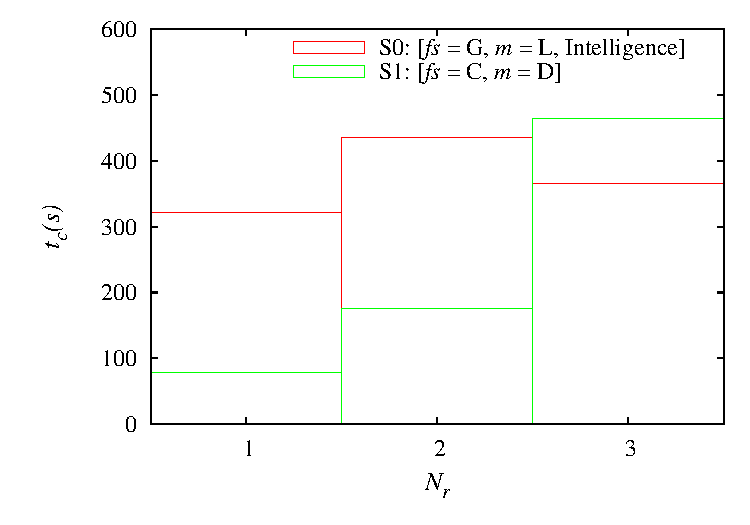
\includegraphics[scale=0.48]{data/graphs/NumberResourcesFigure}
\label{Fig:CloudStoreVsGridFTP:a}
}
\subfigure[$(c_s, N_c, M_c) = (287 MB, 8, C5)$]
{
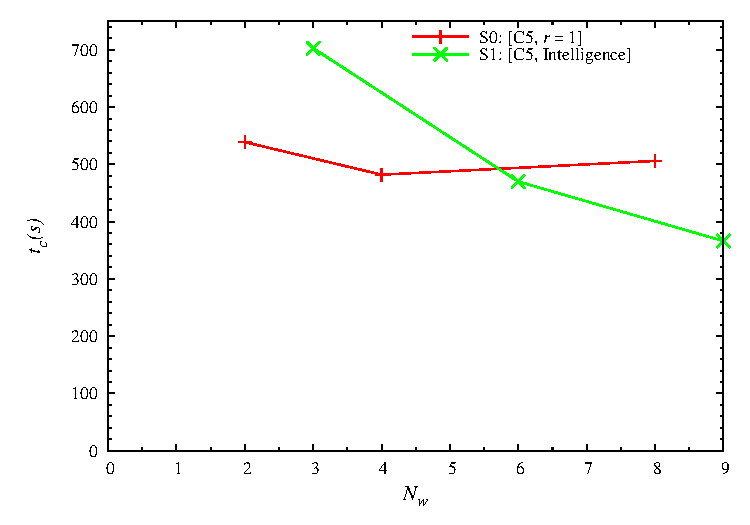
\includegraphics[scale=0.48]{data/graphs/CloudStoreVsGridFTPFigure}
\label{Fig:CloudStoreVsGridFTP:b}
}
\caption{\textit{Figure \ref{Fig:CloudStoreVsGridFTP:a}
 shows optimal times we achieved
for a given number of resources $(N_{r})$. These optimal times do not vary much for our intelligent method, while for CloudStore they improve by adding number of resources (up to three). Figure \ref{Fig:CloudStoreVsGridFTP:b}
demonstrates performance with three resources for both GridFTP and
CloudStore. The three resources compute and have data stores. Performance using CloudStore remains about constant for two, four and eight workers, while our Intelligent approach improved its performance with the number of workers.}}
\label{Fig:CloudStoreVsGridFTP}
\end{center}
\end{figure}

%\section{Analysis}

Overall, the use of CloudStore decreases the time to completion
($t_c$) compared to the intelligent and the local approaches. Our
simple intelligent approach did not performed as well as CloudStore, but
works better than the local tests. For the parameters we used, the
introduction of more workers, up to 8 in our case, decreases the time of
completion; however, for the case of a single machine performing as both
master and workers, we hit an I/O bound, probably caused by the network.
For all of our approaches, GridFTP, Intelligent, and CloudStore, we find
the time to completion for three cases: a single machine is the master
and the workers, one machine does the computing while another has the
data stored, and the case when we spread the data into both machines,
while both of them compute.  In all of our three approaches, the case of
a single machine, shows the least $t_c$. In the case of two machines,
having the data in one, and computing in the other one, increases the
time to completion. By splitting the data in both of the machines, and
computing in both, we decrease $t_c$. We then added another case, all
the data in each of machines, and computing in both. This decreases the
time even further, but not to the point of the local computations;
perhaps, all the approaches are not guaranteed to use the data in the
machine the job is being run, even thought the data is in both machines.

???For our three cases,  $t_c$ may be bounded, and decrease to $t_c$(single machine) as  the number of workers ($N_w$) increases, up to a critical $N_w$, after which $T_c$ will increase due to worker coordination overhead.





\section{Analysis}

Overall, the use of CloudStore decreases the time to completion
($t_c$) compared to the intelligent and the local approaches. Our
simple intelligent approach did not performed as well as CloudStore, but
works better than the local tests. For the parameters we used, the
introduction of more workers, up to 8 in our case, decreases the time of
completion; however, for the case of a single machine performing as both
master and workers, we hit an I/O bound, probably caused by the network.
For all of our approaches, GridFTP, Intelligent, and CloudStore, we find
the time to completion for three cases: a single machine is the master
and the workers, one machine does the computing while another has the
data stored, and the case when we spread the data into both machines,
while both of them compute.  In all of our three approaches, the case of
a single machine, shows the least $t_c$. In the case of two machines,
having the data in one, and computing in the other one, increases the
time to completion. By splitting the data in both of the machines, and
computing in both, we decrease $t_c$. We then added another case, all
the data in each of machines, and computing in both. This decreases the
time even further, but not to the point of the local computations;
perhaps, all the approaches are not guaranteed to use the data in the
machine the job is being run, even thought the data is in both machines.

For our three cases,  $t_c$ may be bounded, and decrease to $t_c$(single
machine) as  the number of workers ($N_w$) increases, up to a critical
$N_w$, after which $T_c$ will increase due to worker coordination
overhead.




\section{Conclusion} Our results show that a DFS greatly changes the
performance of a distributed application in a positive manner. Our
experiments that utilised the DFS to access and store data outperformed
their gridFTP counterparts by an order of magnitude in most cases. Our
results also indicate that the DFS scales better as file sizes and
number of files grow, although both seem to scale linearly. Before any
conclusions may be drawn, there are issues that need to be addressed.
Our application utilised SAGA to access DFS based and gridFTP based
files. There is an overhead that SAGA introduces.  .  In addition, we
were unable to utilise our entire distributed system, using at most 8
jobs to handle our work.  With a replication level of two in the DFS,
data was almost certainly co-located with the computational resource. In
the second experiment, utilizing information from first staging the
network did improve upon the results of the naive first experiment, but
still did not approach the DFS's performance levels.

Distributed filesystems are important abstractions for a data-intensive
distributed application developers to consider. It also appears that
staging is worth the time required to build a graph representing the
network. Also to note, the second experiment is also naive in the way
that it attempts to optimise data and work assignments. Our staging
only performed pings, not data transfer trials or reliability tests. A
job could have low latency, but poor bandwidth. Perhaps CloudStore's
performance can be attributed to recent work that has shown that data in
large scale distributed applications tends to be accessed together,
despite being seemingly unrelated in the input data-set. Such
correlation in data-access has been observed elsewhere, and specific
abstractions to support the access of ``aggregation of such files'' has
been referred to as a filecule, an application specific group of
files~\cite{filecule}. Attempting to determine if analogous
abstractions could enhance performance for the All-Pair application
could be interesting. In a DFS, however, if the data store is also
capable of data processing, then the DFS is placing commonly used files
together on machines needing them for work; in essence, the DFS is
finding these groups for the developer. The fault tolerance, for which
distributed filesystems are already well renowned for, also has added
benefits to grid application developers in terms of performance. The
distributed application does not have to be aware of where data has been
copied to previously when assigning work; the distributed filesystem
uses the best replica when data is being accessed.

{\bf Acknowledgment:} Important funding for SAGA has been provided by
the UK EPSRC grant number GR/D0766171/1 (via OMII-UK) and HPCOPS
NSF-OCI 0710874. SJ acknowledges the e-Science Institute, Edinburgh
for supporting the research theme, ``Distributed Programming
Abstractions'' and theme members for shaping many important
ideas. This work has also been made possible thanks to the internal
resources of the Center for Computation \& Technology at Louisiana
State University and computer resources provided by LONI. 

%\bibliographystyle{IEEEtran}
\bibliographystyle{kluwer} 
\bibliography{data_intensive_paper}
\end{document}
